\documentclass{article}
\usepackage{indentfirst}     
\usepackage{setspace}        
\usepackage[top=1in, bottom=1in, left=1.25in, right=1.25in]{geometry} 
\usepackage{amsmath}
\usepackage{color}
\usepackage{graphicx}
\usepackage{float}
\usepackage{fancyhdr}
\usepackage{hyperref}
\usepackage{mathtools}
\usepackage{amsfonts}
\usepackage{subcaption}

\title{Note on the Heterogeneous Agent Model: Aiyagari (1994)}
\author{Yanran Guo}
\date{June, 2018} 
\begin{document}
\begin{spacing}{1.5}
\maketitle

\section*{Overview}
The purpose of this note is to explain the details of the algorithm of the standard heterogeneous agents model developed by Aiyagari (1994, JPE).\\
The main features of the basic Aiyagari model are
\begin{itemize}
\item There are mass of households. 
\item Households are ex-ante homogeneous bu ex-post heterogeneous, depending on the history of realization of idiosyncratic shocks. In Aiyagari (1994), labor income shock is the only shock.
\item There is only one asset (risk-free asset or capital) that are traded.
\item Hence, households cannot fully insure away their idiosyncratic risks. They can only self-insure by saving.
\item Only the stationary equilibrium is studied: all aggregates don't vary.
\item Prices (wage and interest rate) are determined competitively $\rightarrow$ Use prices to clear markets.
\end{itemize}
\newpage



%%%%%%%%%%%%%%%%%%%%%%%%%%%%%%%%%%%%%%%%%%%%%%%%%%%%%%%%%%%%%%%%%%%%%%%%%%%
\section{Model}
\setlength{\parindent}{2em}
\subsection{Household Problem}
\begin{itemize}
\item Time is discrete. 
\item There are a continuum of households. Total measure of households is normalized to one. Each household has preference
\begin{align*}
\mathbb{E}_0\sum_{t=0}^{\infty}\beta^tu(c_t)
\end{align*}
where $u(c)=\frac{c^{1-\sigma}}{1-\sigma}$
\item Households are endowed with capital $k_0$ initially and one unit of time in each period. Households spend all of their time in working, since leisure is not valued.
\item Households can hold capital $k\geq\phi$ which yields return $r_t$ in period $t$. $\phi$ is the borrowing constraint.
\item A household's labor income in period $t$ is $w_ts_t$ where $w_t$ is the wage for efficiency unit of labor. $s_t$ is idiosyncratic labor productivity shock following a Markov chain $(S,\Pi)$. $S=\{s_1<s_2<...<s_n\}$, each one is a realization of labor productivity. An element of $\Pi$, $\pi_{ii'}$ represents the transition probability $\pi_{ii'}=prob(s_{t+1}=s_{i'}|s_t=s_i)$. $s_t$ of each household is independent of others' $s_t$.
\item Recursive formulation of household problem
\begin{align*}
&V(k,s)=max_{c,k'}{ \ u(c)+\beta\sum_{s'}\pi(s'|s)V(k',s') }\\
&\text{subject to}\\
&c+k'=ws+(1+r)k\\
&c\geq0\\
&k'\geq\phi\\
\end{align*}
\end{itemize}

\subsection{Firm}
There is a representative firm which has access to a CRS technology
\begin{align*}
Y_t=ZK_t^{\alpha}N_t^{1-\alpha}
\end{align*}
where $K_t$ is capital input and $N_t$ is labor input. Firm rents inputs in competitive markets. Capital depreciates at a constant rate $\delta$. Hence, the firm FOCs are
\begin{align*}
&w_t=(1-\alpha)ZK_t^{\alpha}N_t^{-\alpha}\\
&r_t=\alpha ZK_t^{\alpha-1}N_t^{1-\alpha}-\delta\\
\end{align*}

\subsection{Define Recursive Competitive Equilibrium}
A recursive competitive equilibrium consists of prices $r(\mu)$, $w(\mu)$, value function $V(k,s,\mu)$, policy functions $g_k(k,s,\mu)$ and $g_c(k,s,\mu)$, type distribution of households $\mu(k,s)$, and aggregate capital $K(\mu)$ and aggregate labor supply $L(\mu)$, such that
\begin{itemize}
\item Household optimization:\\
Given prices, the value function $V(k,s,\mu)$ is a solution to the household's optimization problem, and $g_k(k,s,\mu)$, $g_c(k,s,\mu)$ are associated policy functions.
\item Firm optimization:
\begin{align*}
&w=(1-\alpha)ZK^{\alpha}N^{-\alpha}\\
&r=\alpha ZK^{\alpha-1}N^{1-\alpha}-\delta\\
\end{align*}
\item Law of motion for $\mu$
\begin{align*}
\mu'(k',s')=\sum_k\sum_s \mu(k,s)\pi(s'|s)\textbf{1}_{{k'=g_k(k,s)}}
\end{align*}
\item Markets clear
\begin{align*}
&\text{Goods: } Y=\int c d\mu+K'-(1-\delta)K\\
&\text{Labor: } N=\int s d\mu\\
&\text{Capital: } K=\int k d\mu\\
\end{align*}
\end{itemize}
\newpage



%%%%%%%%%%%%%%%%%%%%%%%%%%%%%%%%%%%%%%%%%%%%%%%%%%%%%%%%%%%%%%%%%%%%%%%%%%%
\section{Algorithm}
\setlength{\parindent}{2em}
Only the stationary equilibrium is studied.
\begin{enumerate}
\item Guess aggregate $K^d$
\item Given $K^d$, solve for $r$ and $w$ using firm FOCs. \\
Notice that the aggregate labor supply can be computed exogenously in the stationary equilibrium. If we store the stationary distribution regarding the idiosyncratic shocks as $\{P_i\}_{i=1}^{n}$, the aggregate labor supply in the stationary distribution can be computed as
\begin{align*}
N=\sum_{i=1}^ns_iP_i
\end{align*}
Hence $r$ and $w$ are functions of $K$.
\item Given prices, solve household problem using value function iteration to get policy function for $k'$, $g_k(k,s)$
\item Compute the stationary distribution $\mu$
\begin{enumerate}
\item Make an initial guess at the stationary distribution $\mu^0$. A convenient one is uniform distribution. Hence $\mu^0(k,s)=\frac{1}{n_k\times n_s}$ for all $(k,s)$ on the grid.
\item Given initial guess $\mu^0$, compute $\mu^1(k,s)=T^*\mu^0(k,s)$ for all $(k,s)$ on the grid. Given the decision rule obtained in the last step, $g_k(k,s)$, and setting $\mu^1(k,s)=0$ at the start of each new iteration before looping through all $k$, $s$, $s'$, $\mu^1$ can be computed by accumulation. That is, for each triple $(k,s,s')$
\begin{align*}
\mu^1(g_k(k,s),s')=\mu^1(g_k(k,s),s')+\mu^0(k,s)\pi(s'|s)
\end{align*}
Note that the expression above is pseudo-code. The $\mu^1$ term on the RHS represents the value up until the last point in the loop through all $(k,s,s')$, while $\mu^1$ term on the LHS is the new value which includes this $(k,s,s')$.
\item Compute the sup-norm metric $sup_{(k,s)}|\mu^0(k,s)-\mu^1(k,s)|$
\item If the convergence metric from Step-c is within tolerance, exit the loop and set $\mu^1=\mu^*$. Otherwise, set $\mu^0=\mu^1$ and repeat Step-b and c.
\end{enumerate}
\item With the policy function obtained in Step-3 and the stationary distribution obtained in Step-4, compute the aggregate capital supply
\begin{align*}
K^s=\int k d\mu
\end{align*}
\item Define excess capital demand as $\Phi=K^d-K^s$
\item $K^s$ is computed using policy function $g_k(k,s)$ and stationary distribution $\mu(k,s)$, which are computed given prices. And since the prices are functions of our guess for aggregate capital $K^d$, hence $K^s$ depends on $K^d$. Therefore, $\Phi=K^d-K^s$ is a function of $K^d$. Then use `fsolve' to get the the solution for $K^d$\\
\end{enumerate}

\subsection*{A summary of the functions I used to compute the stationary equilibrium of Aiyagari model}
\begin{figure}[!htb]
\centering
\vspace{-2cm}
\hspace*{2cm}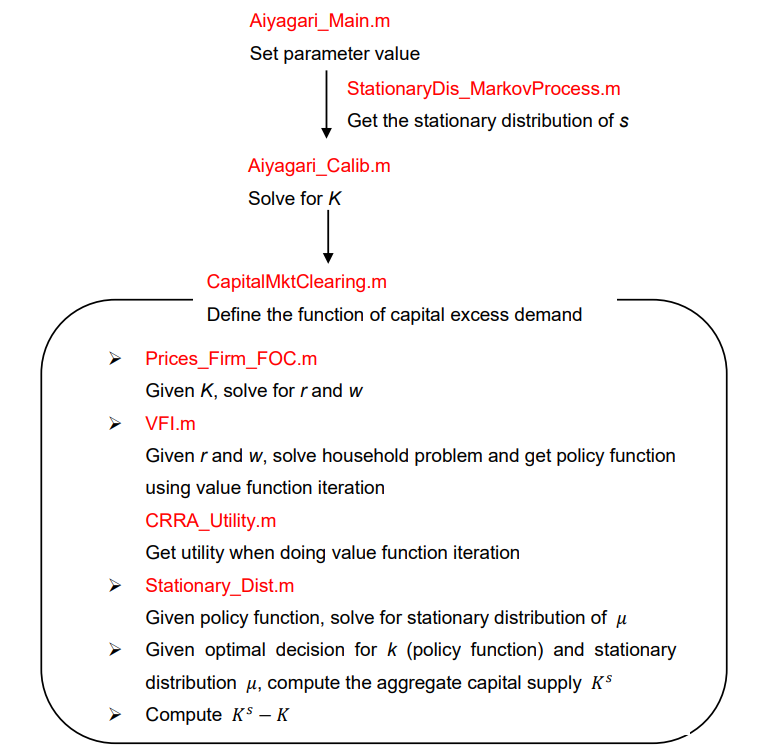
\includegraphics[width=\textwidth,natwidth=450,natheight=430]{readme1.png}\hspace*{-2cm}\\
\end{figure}
\noindent
\textbf{Additional Exercise:} The above functions generate the household's policy functions and value function. Then I simulate $N$ households for $T$ periods to construct Aiyagari (1994) model economy using function file \textcolor{red}{HHSimulation.m}

















\end{spacing}
\end{document}